%%%%%%%%%%%%%%%%%%%%%%% 需求分析 %%%%%%%%%%%%%%%%%%%%%%%%%%%%%%%%%%%%%%%%%%
\chapter{需求分析}
%定义,过去的研究和现在的研究,意义,与图像分割的不同,going deeper
\label{cha:demand_analysis}
\section{问题陈述}

我们将采用C/S架构,建立一个连接微供应商和订购商之间的一个中间平台“鲜天下”。通过该平台,我们得以实现这样的目标:聚合小生厂商的生产力以满足大厂家的订单需求,规模化效应减少运行成本,通过可靠的授信模型为小生厂商提供合适额度的贷款以解决成本问题。

在订购商对虾有较大的需求时,通过“鲜天下”平台,订购商能够在该平台发起订单并支付定金,并实时查看该订单的提交情况与完成情况,如果订单被平台所接受并完成,订购商需要向平台支付剩余款项。

微供应商可以在“鲜天下”平台上注册申请成为认证微供应商,并能够从平台中获得订单。完成订单后,还能够从平台中得到相应款项。同时,根据自己需要,微供应商还可以从“鲜天下”平台申请不超过信用额度的贷款,以此来解决成本问题。

为确保微供应商与订购商之间的协作安全,平台管理人员会对平台所接收到的来自订购商的订单进行审核,并确定是否接受该订单。若接受该订单,平台需要将该订单拆分成多个小订单,并且推送给合适的小生产商在规定时间内完成。同时,平台还需要监控微供应商完成情况,并及时收取货物并完成订购商的订单要求。为了减少微供应商的生产压力,鼓励更多的微供应商参与到该平台中贡献生产力并获得更高的利润,该平台还会记录微供应商相关数据,并根据这些数据,智能地判断每个微供应商可得到的信用额度,以让微供应商获得贷款,减缓它们的资金压力,释放更多的生产力,同时保证平台资金流的安全与稳定。

“鲜天下”平台运行Unix服务器上,能够自动处理用户的请求,并将相关信息存储于数据库中。由于这些信息涉及订单与资金流,该数据库系统必须保证内部数据的一致性,以保证平台的资金流正常运转。


\section{用例析取}

TODO: 需要修改图片,去做申请额度

对“鲜天下”平台,我们完成了用例析取,图示见\autoref{fig:usecase-main}。

%\usepackage{changepage}
%\usepackage{rotating}
%\usepackage{float}
%\usepackage[section]{placeins}
%\begin{sidewaystable}[!Htp]
\begin{figure}[htp]
    %\begin{adjustwidth}{-1.5cm}{-1cm}
    \centering
    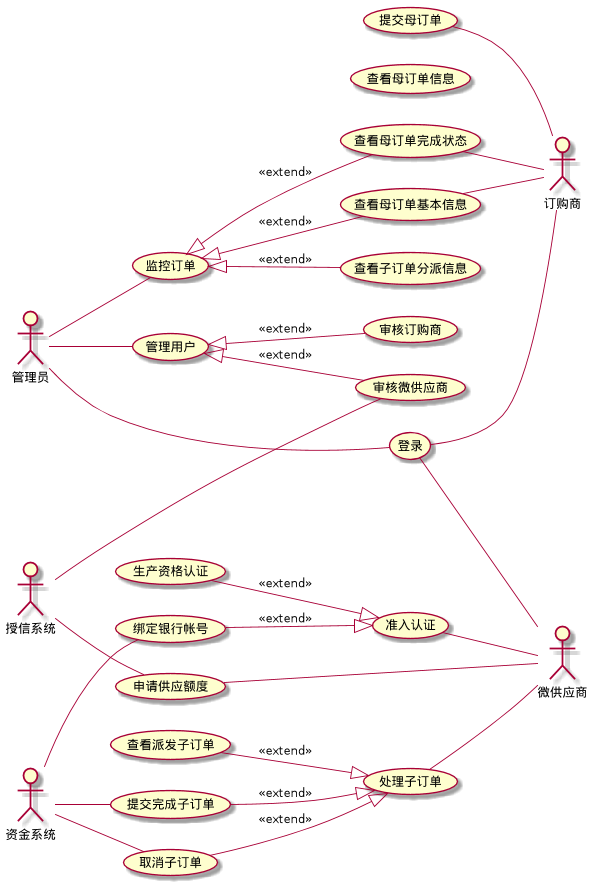
\includegraphics[width=17cm]{figure/usecase/uc_main_ver1.png}
    \caption{“鲜天下平台”用例析取}
    \label{fig:usecase-main}
    %\end{adjustwidth}
\end{figure}


\section{用例规约}




\section{补充规约}

\section{术语表}


